\chapter{Einleitung}

In der Industrie gewinnt Vernetzbarkeit immer mehr an Bedeutung. So lässt sich zum Beispiel durch das Vernetzen von externen Geräten mit den Produktionsmaschinen die Arbeitseffizienz erhöhen. Um diese Kommunikation zu vereinfachen und zu verbessern, wurde das Process Field Network (\gls{profinet}), eine Protokollfamilie, entwickelt.\\
\gls{profinet} setzt auf Ethernet für echtzeitfähige Anwendungen auf, und auf \gls{tcp}/\gls{ip} für langsamere \gls{io} Anwendungen. Durch die immer mehr vernetzten und oft dem Internet zugänglichen Produktionsstätten ist IT-Sicherheit mittlerweile von höchster Bedeutung. \par
Dieses Projekt setzt an dieser Stelle an und soll dem \gls{ids} \gls{snort} ermöglichen, die \gls{profinet} Protokolle zu verstehen und zu verarbeiten. Zu diesem Zweck soll ein \gls{praeprozessor} für \gls{profinet} entwickelt werden. Um dem Benutzer eine Übersicht über die stattfindenden Kommunikationsprozesse zu verschaffen, soll zusätzlich eine \gls{gui} entwickelt werden. Der Kern der \gls{gui} wird ein dargestellter Graph, welcher Kommunikationsteilnehmer im Netzwerk als Knoten darstellt und Kommunikationsbeziehungen als Kanten. Daneben soll es die Möglichkeit geben verschiedene statistische Informationen über den Datenverkehr abzurufen.\\\\
Die Abbildung~\ref{fig:diagram} zeigt im unteren Teil den eben erwähnten \gls{profinet} \gls{praeprozessor}, welcher \gls{snort} die Funktion zum Erkennen und Dekodieren von \gls{profinet} \glspl{paket}n ermöglicht. Die \glspl{paket} werden anschließend per \gls{ipc} zum \gls{programname} Prozess gesendet. Wobei der \gls{programname} Prozess als \textit{CLIENT} die Dienste des \textit{SERVER}s \gls{snort} in Anspruch nimmt (Client-Server-Modell).\\
\Gls{programname} selbst ist nach dem \gls{mvc} Prinzip strukturiert.\\
Das \textit{MODEL} ließt Pakete von der prozessinternen \gls{ipc} Schnittstelle und ordnet sie im verwendeten Datenbestand ein. Der \textit{VIEW} wird über neue Pakete benachrichtigt und präsentiert diese entsprechend auf der \gls{gui}.\\
\textit{Benutzereingaben} im \textit{VIEW} werden dem \textit{CONTROLLER} gemeldet. Dieser erzeugt \textit{Feedback} im \textit{VIEW} welches vom Benutzer wahrgenommen werden kann. Der \textit{CONTROLLER} hat außerdem die Möglichkeit durch Benutzerbefehle oder andere Geschäftslogiken induzierte Manipulationen am \textit{MODEL} vorzunehmen.

\begin{figure}[h]
  \centering
  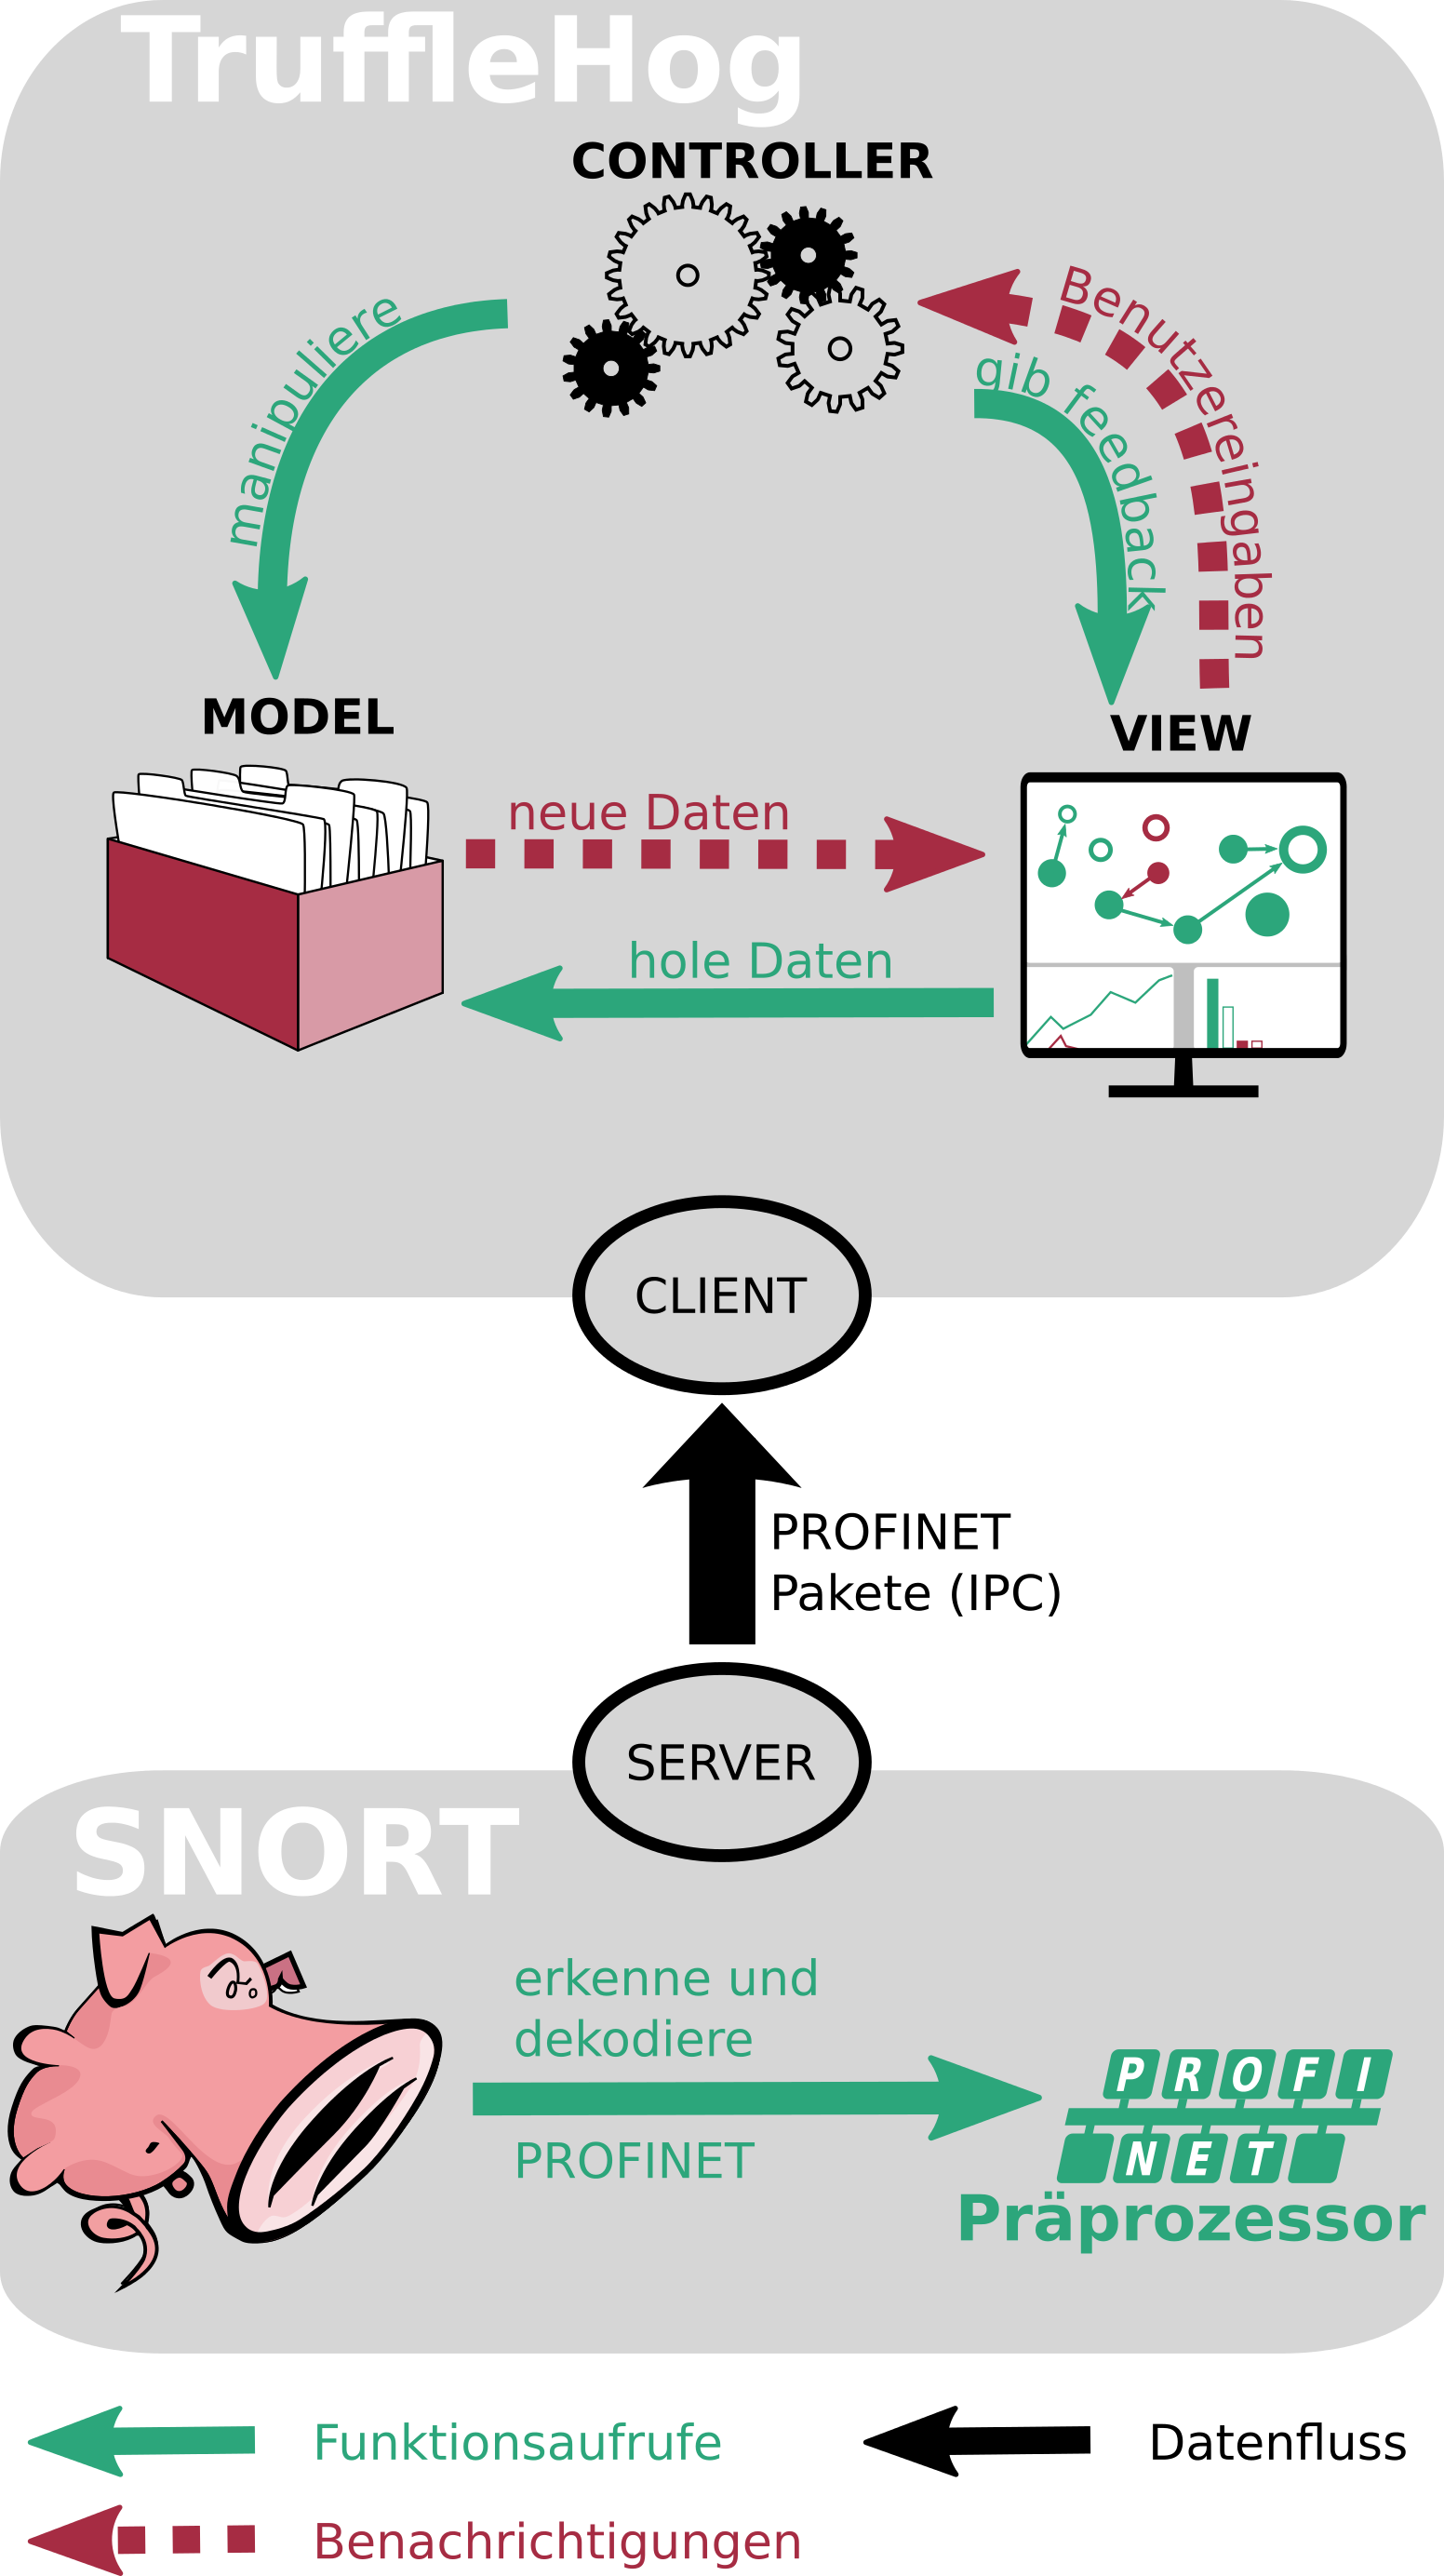
\includegraphics[width=300pt]{../diagrams/intro_diagram/intro_diagram.png}
  \caption[Strukturübersicht des Projekts]{Strukturübersicht des Projekts}\label{fig:diagram}
\end{figure}